
\begin{frame}[c]
 \frametitle{Data integration}
 \framesubtitle{Parameters inference/Principe}
 
\begin{columns}

\begin{column}{0.7\textwidth}
\scalebox{0.9}{
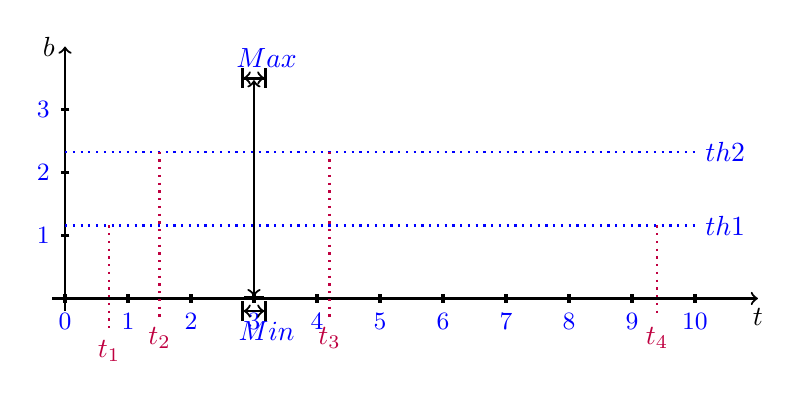
\begin{tikzpicture}[scale = 0.8]
    % Tracé de la parabole
    %\draw[red, domain = -2.2:2.2, smooth] plot (\x, {(\x)^2});
    % Alternative par Gnuplot
    %\draw[red, domain = -2.2:2.2, smooth] plot function{x**2};
    % Lignes tiretées
      \draw[thick, ->] (-.2,0)--(11,0) node[below]{$t$};
     \foreach \t in {0,1,2,3,4,...,10}
      \draw[very thick] (\t,2pt)--(\t,-2pt) node[below,blue]{\small\t};

     \draw[thick, ->] (0,-.2)--(0,4) node[left]{$b$};
     \foreach \y in {1,2,3}
      \draw[very thick] (2pt,\y)--(-2pt,\y) node[left,blue]{\small\y};
      
    \draw[thick] plot[mark=ball,mark size=1pt] file {illustration.txt};
    
    \onslide<2->{
    \draw[thick,|<->|] (2.8,3.5) -- (3.2,3.5) node[above,blue]{$Max$};
    \draw[thick,|<->|] (2.8,-.2) -- (3.2,-.2) node[below,blue]{$Min$};
    }
    \onslide<3->{
    \draw[thick,|<->|] (3,0) -- (3,3.5);
    }
    \onslide<4->{
    \draw[thick,dotted,blue] (0,1.16) -- (10,1.16) node[right]{$th1$}; 
    \draw[thick,dotted,blue] (0,2.33) -- (10,2.33) node[right]{$th2$}; 
    }
    \onslide<5->{
    \draw[thick,dotted,purple] (0.7,1.16) -- (0.7,-.5) node[below]{$t_{1}$};
    }
    \onslide<6->{
    \draw[thick,dotted,purple] (1.5,2.33) -- (1.5,-.3) node[below]{$t_{2}$};
    }
    \onslide<7->{
    \draw[thick,dotted,purple] (4.2,2.33) -- (4.2,-.3) node[below]{$t_{3}$};
    }
    \onslide<8->{
    \draw[thick,dotted,purple] (9.4,1.16) -- (9.4,-.3) node[below]{$t_{4}$};
    }
\end{tikzpicture}
}
%If we assume that $t_{0}=0$,\\
\onslide<5->{$\PHfrappe{a_1}{b_0}{b_1}$ with $r_{1}=\frac{1}{t_{1}-t_{0}}$\\}
\onslide<6->{$\PHfrappe{a_1}{b_1}{b_2}$ with $r_{2}=\frac{1}{t_{2}-t_{1}}$\\}
\onslide<7->{$\PHfrappe{a_0}{b_2}{b_1}$ with $r_{3}=\frac{1}{t_{3}-t_{2}}$\\}
\onslide<8->{$\PHfrappe{a_0}{b_1}{b_0}$ with $r_{4}=\frac{1}{t_{4}-t_{3}}$\\}
\onslide<8->{The formula to estimate the rate of the dynamics of a component according to it TSD is 
\tval{ \Large {$r_{i}=\frac{1}{t_{i}-t_{i-1}}$}}}
\end{column}

\begin{column}{0.3\textwidth}
\scalebox{0.9}{
 \begin{tikzpicture}[scale=0.8]
\path[use as bounding box] (-1,-1) rectangle (2,2);


\TSort{(0,1)}{b}{3}{r}


\only<5->{\TSort{(2,1)}{a}{2}{l}}
\only<5>{
\THit{a_1}{}{b_0}{.east}{b_1}
%\THit{a_0}{out=-120,in=180,selfhit}{a_0}{.west}{a_1}
\path[bounce]
%\TBounce{a_0}{bend left}{a_1}{.south}
\TBounce{b_0}{bend right}{b_1}{.south}
;
\TState{5}{a_1,b_0}
\TState{5}{a_1,b_1}
}

%deuxième estimation
\only<6>{
\THit{a_1}{}{b_1}{.east}{b_2}
%\THit{a_0}{out=-120,in=180,selfhit}{a_0}{.west}{a_1}
\path[bounce]
%\TBounce{a_0}{bend left}{a_1}{.south}
\TBounce{b_1}{bend right}{b_2}{.south}
;
\TState{6}{a_1,b_1}
\TState{6}{a_1,b_2}
}

%troisième  estimation
\only<7>{
\THit{a_0}{}{b_2}{.east}{b_1}
%\THit{a_0}{out=-120,in=180,selfhit}{a_0}{.west}{a_1}
\path[bounce]
%\TBounce{a_0}{bend left}{a_1}{.south}
\TBounce{b_2}{bend right}{b_1}{.north}
;
\TState{7}{a_0,b_2}
\TState{7}{a_0,b_1}
}

%troisième  estimation
\only<8>{
\THit{a_0}{}{b_1}{.east}{b_0}
%\THit{a_0}{out=-120,in=180,selfhit}{a_0}{.west}{a_1}
\path[bounce]
%\TBounce{a_0}{bend left}{a_1}{.south}
\TBounce{b_1}{bend right}{b_0}{.north}
;
\TState{8}{a_0,b_1}
\TState{8}{a_0,b_0}
}

\end{tikzpicture}
}

\end{column}
\end{columns}
\end{frame}
